The strength of the MIPS processor is its fixed and simple RISC instruction set and its simple and non overlapping pipeline stages. Three types of instructions exist in the set. R-types which is the registry format, I-type which is the immediate format and J-type which is the jump format. These instructions are 32-bit wide in a 32-bit machine and arranged as shown in Figure \ref{fig:ISA}. % Why the fuck does this reference go wrong???

\begin{figure}[!h] 
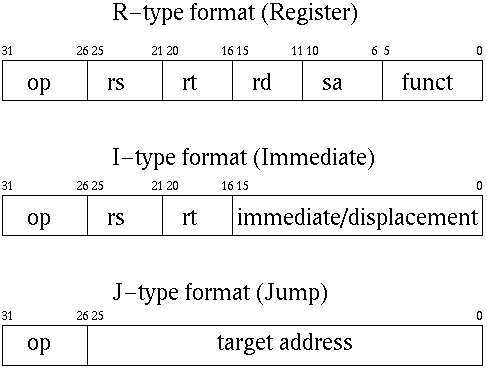
\includegraphics[width=0.45\textwidth]{Images/image.png}
\caption{MIPS instruction types}
\label{fig:ISA}
\end{figure}

In the following section, the theory behind the MIPS processor architecture, and some aspects of processors in general are introduced. Some things were implemented in our processor, while others (such as caching and branch prediction) were unfortunately left out due to time constraints. Most of the theory section is based on \cite{Patterson:2008:COD:1502247} and \cite{CompArch}.

\subsection{Processor Architecture}
In order to speed up modern processors, parallelism has to be exploited. One way to achieve this is through pipelining. By dividing instruction into sub instructions, a new instruction can be started right after the previous sub instruction has finished. The maximum speed up of pipelining is equal to the number of pipeline stages. However, pipelining introduces a number of problems due to dependencies. These problems can be categorized as structural hazards, data hazards and control hazards.

To deal effectively with these hazards, forwarding and branch prediction has to be introduced. Our processor is pipelined into five independent stages and therefore the maximum speed up of our processor compared to the non-pipeline alternative is 5. The five pipeline stages of the MIPS processor is: Instruction fetch, Instruction decode, Execute, Memory access and Write back.

Due to Moore's law, the size and price of semi conductors has decreased dramatically. This has spawned new processor designs which implement parallelism and pipelining. At the same time memory modules have not been evolving at the same pace, making memory one of the biggest bottlenecks in modern computers. Modern processors can process huge amount of data, but without efficient memory, these processors have to stall in order for the memory module to respond.

The ideal memory has a low response time and at the same time an unlimited amount of storage. This is extremely expensive because fast memory is expensive. however it is possible to create an illusion of a big fast memory by introducing memory hierarchy. Because slow memory is cheap, a large part of the memory should be build by slow memory, layers of faster and faster and smaller and smaller memory modules should be build on top of the slower memory modules. The processor should then communicate mostly with upper levels of the memory modules which would decrease latency of the module.

To take advantage of a memory hierarchy the memory should be build with spatial and temporal locality in mind. Spatial locality is a concept of loading data close to the fetched data in to upper level of the memory, whereas temporal locality is a concept of reusing data that has previously been used.

The caches of today which is the upper part of the memory hierarchy are located at the CPU chip. A big part of the CPU chip today is in fact cache in different levels. L1 and L2 caches are usually small memory units, which can only be accessed by one core, while L3 caches are bigger and can be accessed by multiple core depending on the architecture. An example of such a cache hierarchy can be seen in Figure \ref{cache}.

\begin{figure}[!h] 
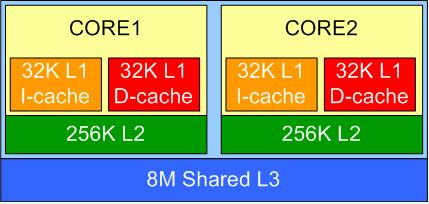
\includegraphics[width=0.45\textwidth]{Images/Cache_level.JPG}
\caption{On chip cache}
\label{cache}
\end{figure}


Main memory is located outside the CPU chip and is the slowest part of the memory hierarchy. A typical modern main memory in a desktop or laptop PC is around 4 to 8 Gb of storage. If there is a cache miss, and data has to be fetched from main memory, the penalty is in the range of thousands of clock cycles depending on the technology. 

In the eighties and nineties processors got more and more advanced, and computer designers only had to think about speed of the components. Pipeline stages and complexity exploded to get that extra speed, and thus the frequency in which the processor operated increased. When the computer designers hit the power wall, a whole new challenge was introduces: how to go fast without dissipating to much power. There is a fixed amount of power that can be dissipated without melting the chip. A processor that runs at 4 GHz but consumes more than double the power of a 2 GHz processor is actually quite often slower. This is because the of parallelism implemented in today's CPUs. The reason computer designers hit the power wall is because of the following equation:

\begin{eqnarray}
\label{Power Dissipation}
P = CV^2f 
\end{eqnarray}

This equation states that the power dissipation is equal to the capacitance times the voltage squared times the switching frequency. Since the voltage level and the capacitance are largely dependent on the CMOS technology used to produce the chip, these are normally outside the control of the hardware designer. However, by lowering the frequency and create more efficient pipeline stages, it is possible to reduce the power consumption without reducing the throughput. 

Because power dissipation is the limiting factor units can be shut down when they are not used. This can be done by removing the clock signal or the power to the unit. 